\documentclass[tikz,border=3pt,convert={density=600,outext=.png}]{standalone}
%\documentclass[tikz,border=3pt]{standalone}

\usepackage[utf8]{inputenc} % utf8 encoding

\usepackage{amsmath} % nice math symbols
     

\usepackage{tikz}
\usetikzlibrary{shapes,positioning,calc}

% TikZ styles for drawing

\begin{document}
	
	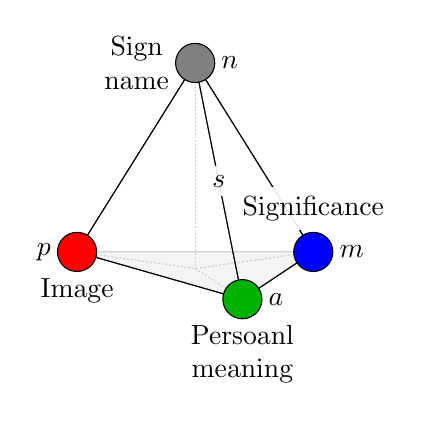
\begin{tikzpicture}[join=round,scale=3.0,node distance = -0.05]
		\tikzstyle{sign_comp}=[draw, circle, scale=1.5];
		\tikzstyle{label}=[align=center,fill=white,opacity=0.9,text opacity=1];
		\tikzstyle{coord_cine}=[dash pattern=on 0.7 off 0.7];
		
		\filldraw[fill=white] (0.0,0.2) -- (0.5,1.0) -- (1.0,0.2) -- cycle;
		\filldraw[fill=black!20] (0.0,0.2) -- (0.7,0.0) -- (1.0,0.2) -- cycle;

		\draw[coord_cine] (0.5,1.0) -- (0.5,0.13);
		\draw[coord_cine] (0.0,0.2) -- (0.5,0.13);
		\draw[coord_cine] (0.7,0.0) -- (0.5,0.13);
		\draw[coord_cine] (1.0,0.2) -- (0.5,0.13);

		\filldraw[fill=white,fill opacity=0.8] (0.0,0.2) -- (0.5,1.0) -- (0.7,0.0) -- cycle;
		\filldraw[fill=white,fill opacity=0.8] (0.7,0.0) -- (0.5,1.0) -- (1.0,0.2) -- cycle;
				
		\node[sign_comp, fill=red] (s_p) at (0.0,0.2) {};
		\node[sign_comp, fill=blue] (s_m) at (1.0,0.2) {};
		\node[sign_comp, fill=gray] (s_n) at (0.5,1.0) {};
		\node[sign_comp, fill=green!70!black] (s_a) at (0.7,0.0) {};
		
		\node[left = of s_p] {$p$};
		\node[below = of s_p] {Image};
		\node[right = of s_m] {$m$};
		\node[label,node distance = 0.01, above = of s_m] {Significance};
		\node[right = of s_n] {$n$};
		\node[left = of s_n,align=center] {Sign\\name};
		\node[right = of s_a] {$a$};
		\node[below = of s_a,align=center] {Persoanl\\meaning};
		
		\node[label] at ($(s_n)!0.5!(s_a)$) {$s$};
		
	\end{tikzpicture}

\end{document}